\documentclass[12pt]{article}
\usepackage[utf8]{inputenc}
\usepackage[T1]{fontenc}
\usepackage[a4paper]{geometry}
\geometry{hscale=0.80,vscale=0.80,centering}
\usepackage{amsmath}
\usepackage{amsthm}
\usepackage{stmaryrd}
\newcommand{\subsubsubsection}[1]{\paragraph{#1}\mbox{}\\}
\setcounter{secnumdepth}{4}
\setcounter{tocdepth}{4}
\usepackage{amssymb}
\usepackage{multicol}
\usepackage{breqn}
\usepackage{fancyhdr}
\pagestyle{fancy}
%\fancyhf{}
%\rhead{P-ANDROIDE}
%\lhead{David PINAUD | Emilie BIEGAS}
%\rfoot{Page \thepage}
\pagestyle{fancy}
\fancyhf{}
\fancyhead[LE,RO]{David PINAUD | Emilie BIEGAS}
\fancyhead[RE,LO]{P-ANDROIDE}
\fancyfoot[CE,CO]{\leftmark}
\fancyfoot[LE,RO]{\thepage}
\renewcommand{\headrulewidth}{1pt}
\renewcommand{\footrulewidth}{1pt}

\usepackage{graphicx}
\usepackage{subcaption}
\usepackage[affil-it]{authblk}
\usepackage{pdfpages}
\newcommand{\Mod}[1]{\ (\mathrm{mod}\ #1)}
\usepackage{hyperref}
\begin{document}

\begin{titlepage}

\newcommand{\HRule}{\rule{\linewidth}{0.5mm}} % Defines a new command for the horizontal lines, change thickness here

\center % Center everything on the page
 
%----------------------------------------------------------------------------------------
%	HEADING SECTIONS
%----------------------------------------------------------------------------------------

\textsc{\LARGE Sorbonne Université}\\[1.5cm] % Name of your university/college
\textsc{\Large Projet P-A.N.D.R.O.I.D.E}\\[0.5cm] % Major heading such as course name
\textsc{\large Dépôt Github : \url{https://git.io/J39ZB}}\\[0.5cm] % Minor heading such as course title

%----------------------------------------------------------------------------------------
%	TITLE SECTION
%----------------------------------------------------------------------------------------

\HRule \\[0.4cm]
{ \huge \bfseries Branch and Bound pour les Diagrammes d'influence}\\[0.4cm] % Title of your document
\HRule \\[1.5cm]
 
%----------------------------------------------------------------------------------------
%	AUTHOR SECTION
%----------------------------------------------------------------------------------------

\begin{minipage}{0.4\textwidth}
\begin{flushleft} \large
\emph{Auteurs:}\\
David \textsc{PINAUD} % Your name

Emilie \textsc{BIEGAS} % Your name
\end{flushleft}
\end{minipage}
~
\begin{minipage}{0.4\textwidth}
\begin{flushright} \large
\emph{Encadrant:} \\
M. Pierre-Henri \textsc{WUILLEMIN} % Supervisor's Name
\end{flushright}
\end{minipage}\\[2cm]

% If you don't want a supervisor, uncomment the two lines below and remove the section above
%\Large \emph{Author:}\\
%John \textsc{Smith}\\[3cm] % Your name

%----------------------------------------------------------------------------------------
%	DATE SECTION
%----------------------------------------------------------------------------------------

{\large 8 Mai 2021}\\[2cm] % Date, change the \today to a set date if you want to be precise

%----------------------------------------------------------------------------------------
%	LOGO SECTION
%----------------------------------------------------------------------------------------


\includegraphics[scale=0.5]{logo.png}\\[1cm] % Include a department/university logo - this will require the graphicx package
 
%----------------------------------------------------------------------------------------

\vfill % Fill the rest of the page with whitespace

\end{titlepage}

\renewcommand{\contentsname}{Table des Matières}
\pagebreak
\tableofcontents
\pagebreak

\section{Introduction}

\subsection{Les diagrammes d'influence (ID)}
Un diagramme d'influence est une représentation graphique et mathématique compacte d'une situation de décision. Il s'agit d'une généralisation d'un réseau bayésien, dans lequel non seulement les problèmes d'inférence probabiliste, mais aussi les problèmes de prise de décision peuvent être modélisés et résolus. 
Le diagramme d'influence est une bonne alternative aux arbres de décision qui peuvent devenir extrêmement complexes. En effet, elles permettent de représenter des arbres de décision symétriques de façon compacte. On se place dans ce projet dans le cadre du maximum d'utilité.

Considérons, par exemple, une situation de décision concernant le choix d'une activité (de domaine : sport en plein air ou sport en intérieur) prise selon la prévision météorologique qui dépend, elle, des conditions réelles (leurs domaines est : pluvieux ou ensoleillé). Le diagramme d'influence 1 (a) ci-dessous permet de représenter cette situation et est équivalent à l'arbre de décision de la figure 1 (b).

\begin{figure}[ht]
\centering
\begin{subfigure}{.5\textwidth}
  \centering
  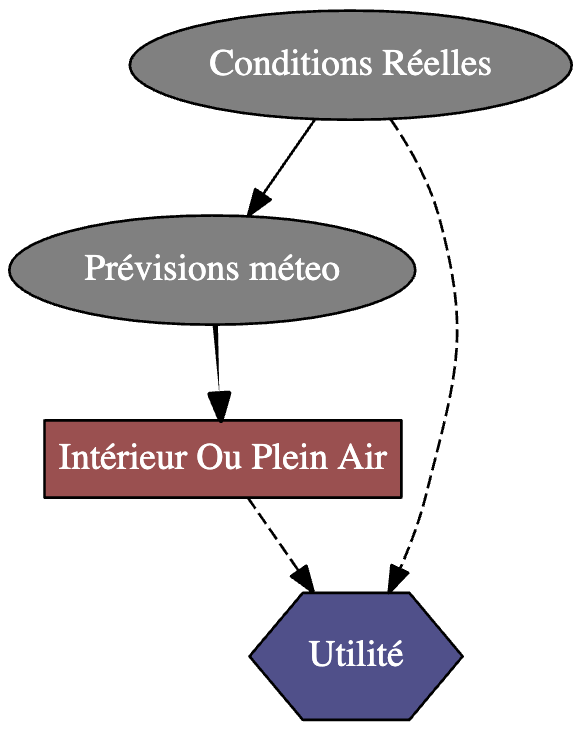
\includegraphics[width=.5\linewidth]{docs/ressources_rapport/exempleID_SIMPLE.png}
  \caption{Diagramme d'influence}
  \label{fig:sub1}
\end{subfigure}%
\begin{subfigure}{.5\textwidth}
  \centering
  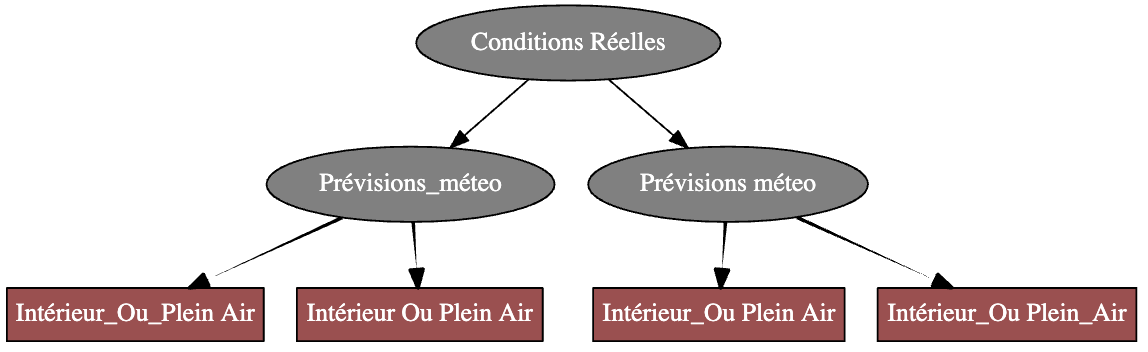
\includegraphics[width=1.2\linewidth]{docs/ressources_rapport/exempleArbreDecision.png}
  \caption{L'arbre de décision symétrique associé}
  \label{fig:sub2}
\end{subfigure}
\caption{ID et Arbre de décision}
\label{fig:test}
\end{figure}

Plus précisément, les diagrammes d'influence (ID) sont des graphes dirigés acycliques présentant trois types de nœuds. Les nœuds de \textit{chance}, illustrés graphiquement par un ovale, représentent des variables aléatoire (dont le domaine est fini et non vide). 
Les nœuds de \textit{décision}, illustrés graphiquement par un rectangle, représentent des variables de décision (dont le domaine est fini et non vide) tandis que les nœuds d'\textit{utilité}, illustrés graphiquement par un octogone ou un hexagone, représentent une fonction d'utilité locale exprimant la préférence.
Lorsqu'il y a plusieurs nœuds d'utilité, l'utilité totale en est la somme (c'est une décomposition partiellement additive de l'utilité).

Les arcs de ce graphe représentent une dépendance entre les nœuds et ont une signification différente en fonction du type de nœud à son extrémité.
En effet, si un arc pointe vers un nœud de chance, cela représente une dépendance probabiliste; si il pointe vers un nœud de décision, il a un but informatif; enfin, si il pointe vers un nœud d'utilité, il représente une dépendance fonctionnelle.

\bigbreak
Les IDs respectent deux hypothèses, une hypothèse de régularité (les décisions sont ordonnées dans le temps) et une hypothèse dite non-oubliant (chaque décision est conditionnée par toutes les observations de décisions antérieures).
L'ensemble des instanciations des nœuds de chance pour les décisions antérieures d'une certaine décision est appelé l'\textit{historique}.
\\\\


\subsection{Les LIMIDs}
Les \textit{LImited-Memory Influence-Diagrams} (LIMIDs) sont des diagrammes d'influence qui assouplissent les deux hypothèses précédemment citées. 
 
Tout d'abord, les LIMIDs assouplissent l'hypothèse non-oubliant de manière à conditionner une décision sur un nombre limité d'observations et de décisions antérieurs pertinentes (pour un compromis qualité/complexité).

Ensuite, assouplir l'hypothèse de régularité permet par exemple de modéliser la coopération de problèmes de décision multi-agents où un agent n'est pas au courant de décision d'autres agents. 
Les IDs forment alors un sous-ensemble des LIMIDs. On peut en voir un exemple ci-dessous.
\begin{figure}[ht]
\centering
\begin{subfigure}{.5\textwidth}
  \centering
  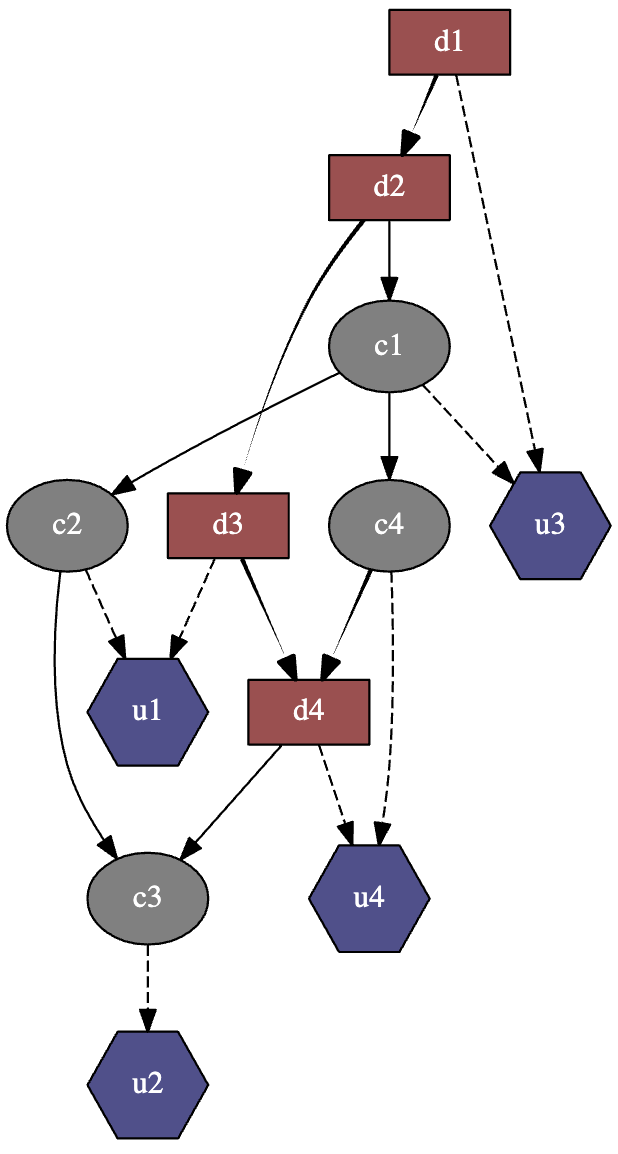
\includegraphics[width=.5\linewidth]{docs/ressources_rapport/ID_LIMID.png}
  \caption{Diagramme d'influence}
  \label{fig:sub3}
\end{subfigure}%
\begin{subfigure}{.5\textwidth}
  \centering
  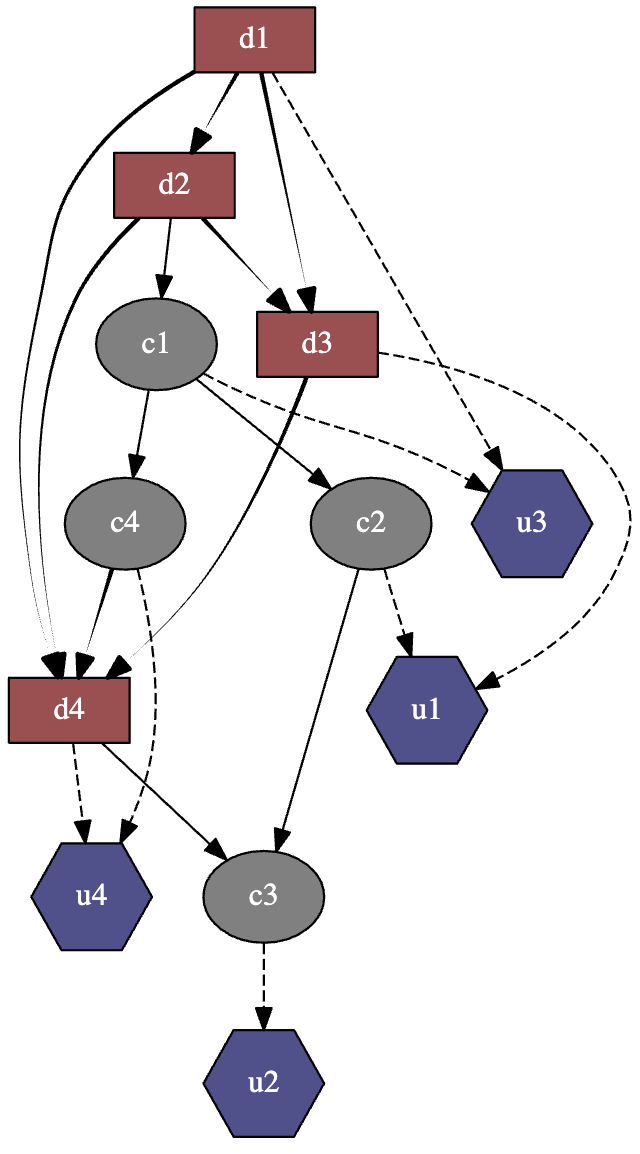
\includegraphics[width=0.5\linewidth]{docs/ressources_rapport/LIMID_ID.png}
  \caption{LIMID associé à l'ID}
  \label{fig:sub4}
\end{subfigure}
\caption{ID et LIMID}
\label{fig:test1}
\end{figure}

\subsection{Limites des implémentations actuelles}

Les méthodes de résolution exactes actuelles de LIMIDs ou IDs sont limités par leur complexité en temps et en espace.
Pour exemple, considérons un ID qui modélise un robot dans un labyrinthe représenté par une matrice $n\times m$ composé de cases \textit{mur}, de cases \textit{libre} et d'une case \textit{objectif}. On représente le labyrinthe comme ci-dessous, les cases grises, blanches, et étoilés étant respectivement les cases \textit{mur}, \textit{libre}, et \textit{objectif}.

\begin{figure}[ht]
\centering
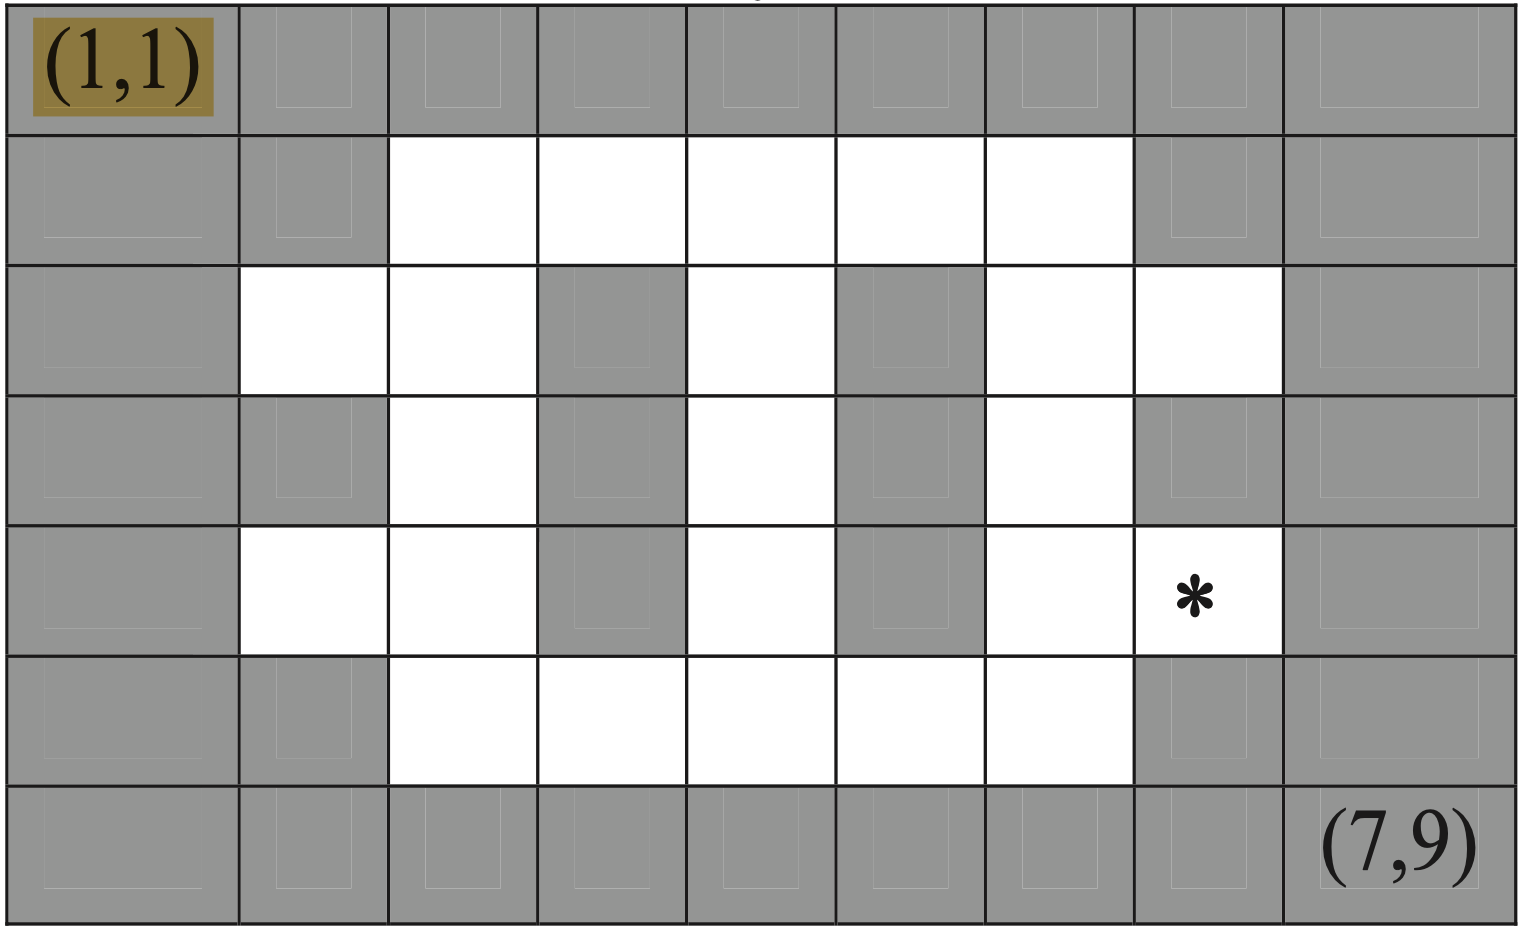
\includegraphics[scale=0.2]{docs/ressources_rapport/MAZE.png}
\caption{Un exemple de représentation d'un labyrinthe $9\times 7$}
\end{figure}
Le robot est initialement placé sur une des cases \textit{libre} et l'objectif du robot est d'atteindre la case \textit{objectif}. 
À chaque étape, le robot peut se déplacer dans toutes les directions (nord, sud, est, ouest et les diagonales) d'une seule case ou choisir de ne pas se déplacer. Il possède quatre capteurs pointés vers les quatre cardinaux qui indiquent au robot la présence d'un mur ou non.
%les probabilités sommes à 1 --> c'est bien une distribution donc pas de mouvement en diagonale possible ?!

À chaque étape, le robot choisit une direction cardinale où faire un pas puis le mouvement du robot suit une mesure de probabilité :
\begin{itemize}
  \item Un pas vers la case voulu a une probabilité $pBouger$ de réussir.
  \item Échouer de bouger survient avec probabilité $pEchecBouger$.
  \item Un pas vers un \textit{mur} a une probabilité de 0.
  \item À chaque étape, il y a une chance que le robot fasse un mouvement erratique :
  \begin{itemize}
        \item Faire un pas vers la droite ou vers la gauche (c'est-à-dire vers l'est ou vers l'ouest si son choix est de se diriger vers le nord), s'il est possible de le faire, survient avec une probabilité de $pCote$ dans chacun des deux cas.
        \item Faire un pas en arrière (c'est-à-dire vers le sud si son choix est de se diriger vers le nord), s'il est possible de le faire, survient avec une probabilité $pArriere$.
        \end{itemize}
  \item Les autres probabilités sont normalisées afin de former une distribution de probabilité.
\end{itemize}

\begin{figure}[ht]
\centering
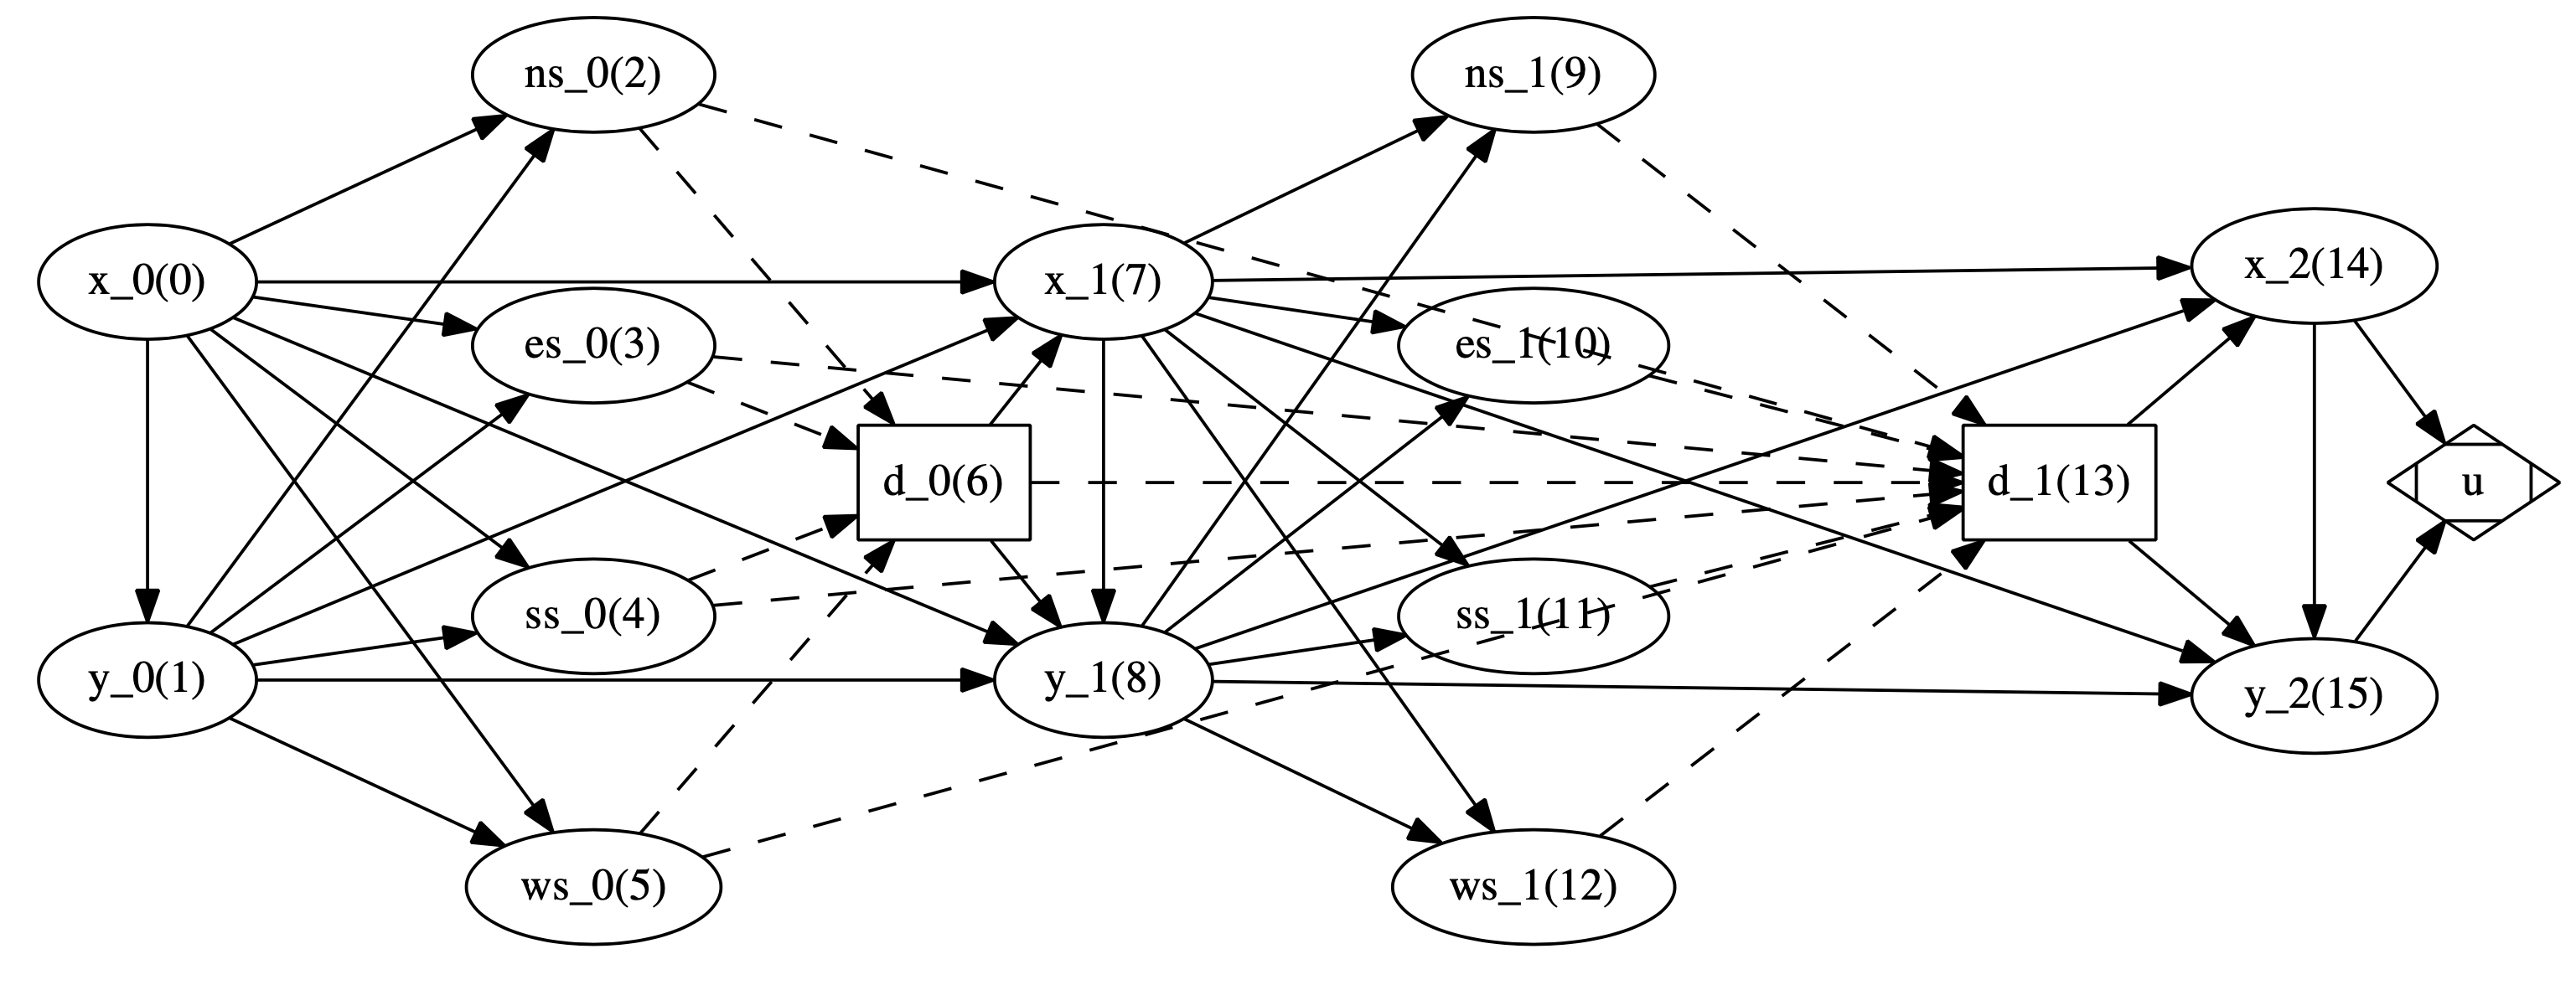
\includegraphics[scale=0.22]{docs/ressources_rapport/IDROBOT.png}
\caption{L'ID modélisant le problème du robot à deux étapes }
\end{figure}

A l'étape $i$, les nœuds de chance $x_i$ et $y_i$ représentent les coordonnées du robot sur la grille, $ns_i, es_i, ss_i, ws_i$ les capteurs du robot dans les sens nord, est, sud et ouest respectivement. Les nœuds $d_i$ sont les nœuds de décision.
Pour visualiser le caractère exponentiel de la complexité en espace, voici un tableau récapitulatif des tailles des arbres de jonctions selon le nombre d'étapes ainsi que les graphes associés.

\bigbreak
\begin{center}
   \begin{tabular}{|p{3cm} || p{3cm} | p{3cm} | }
    \hline
    Nombre d'étapes & Tree-width (largeur de l'arbre) & taille en mémoire de l'arbre (en Go) \\ 
    \hline
    2&11&0,002\\
    \hline
    3&15&0,038\\
    \hline
    4&20&0,787\\
    \hline
    5&24&12\\
    \hline
    6&29&984\\
    \hline
    7&34&76 000\\
    \hline
    8&37&246 000\\
    \hline
    9&42&19 687 000\\
    \hline
    10&46&315 000 000\\
    \hline
   \end{tabular}
\end{center}
 \begin{figure}[ht]
\centering
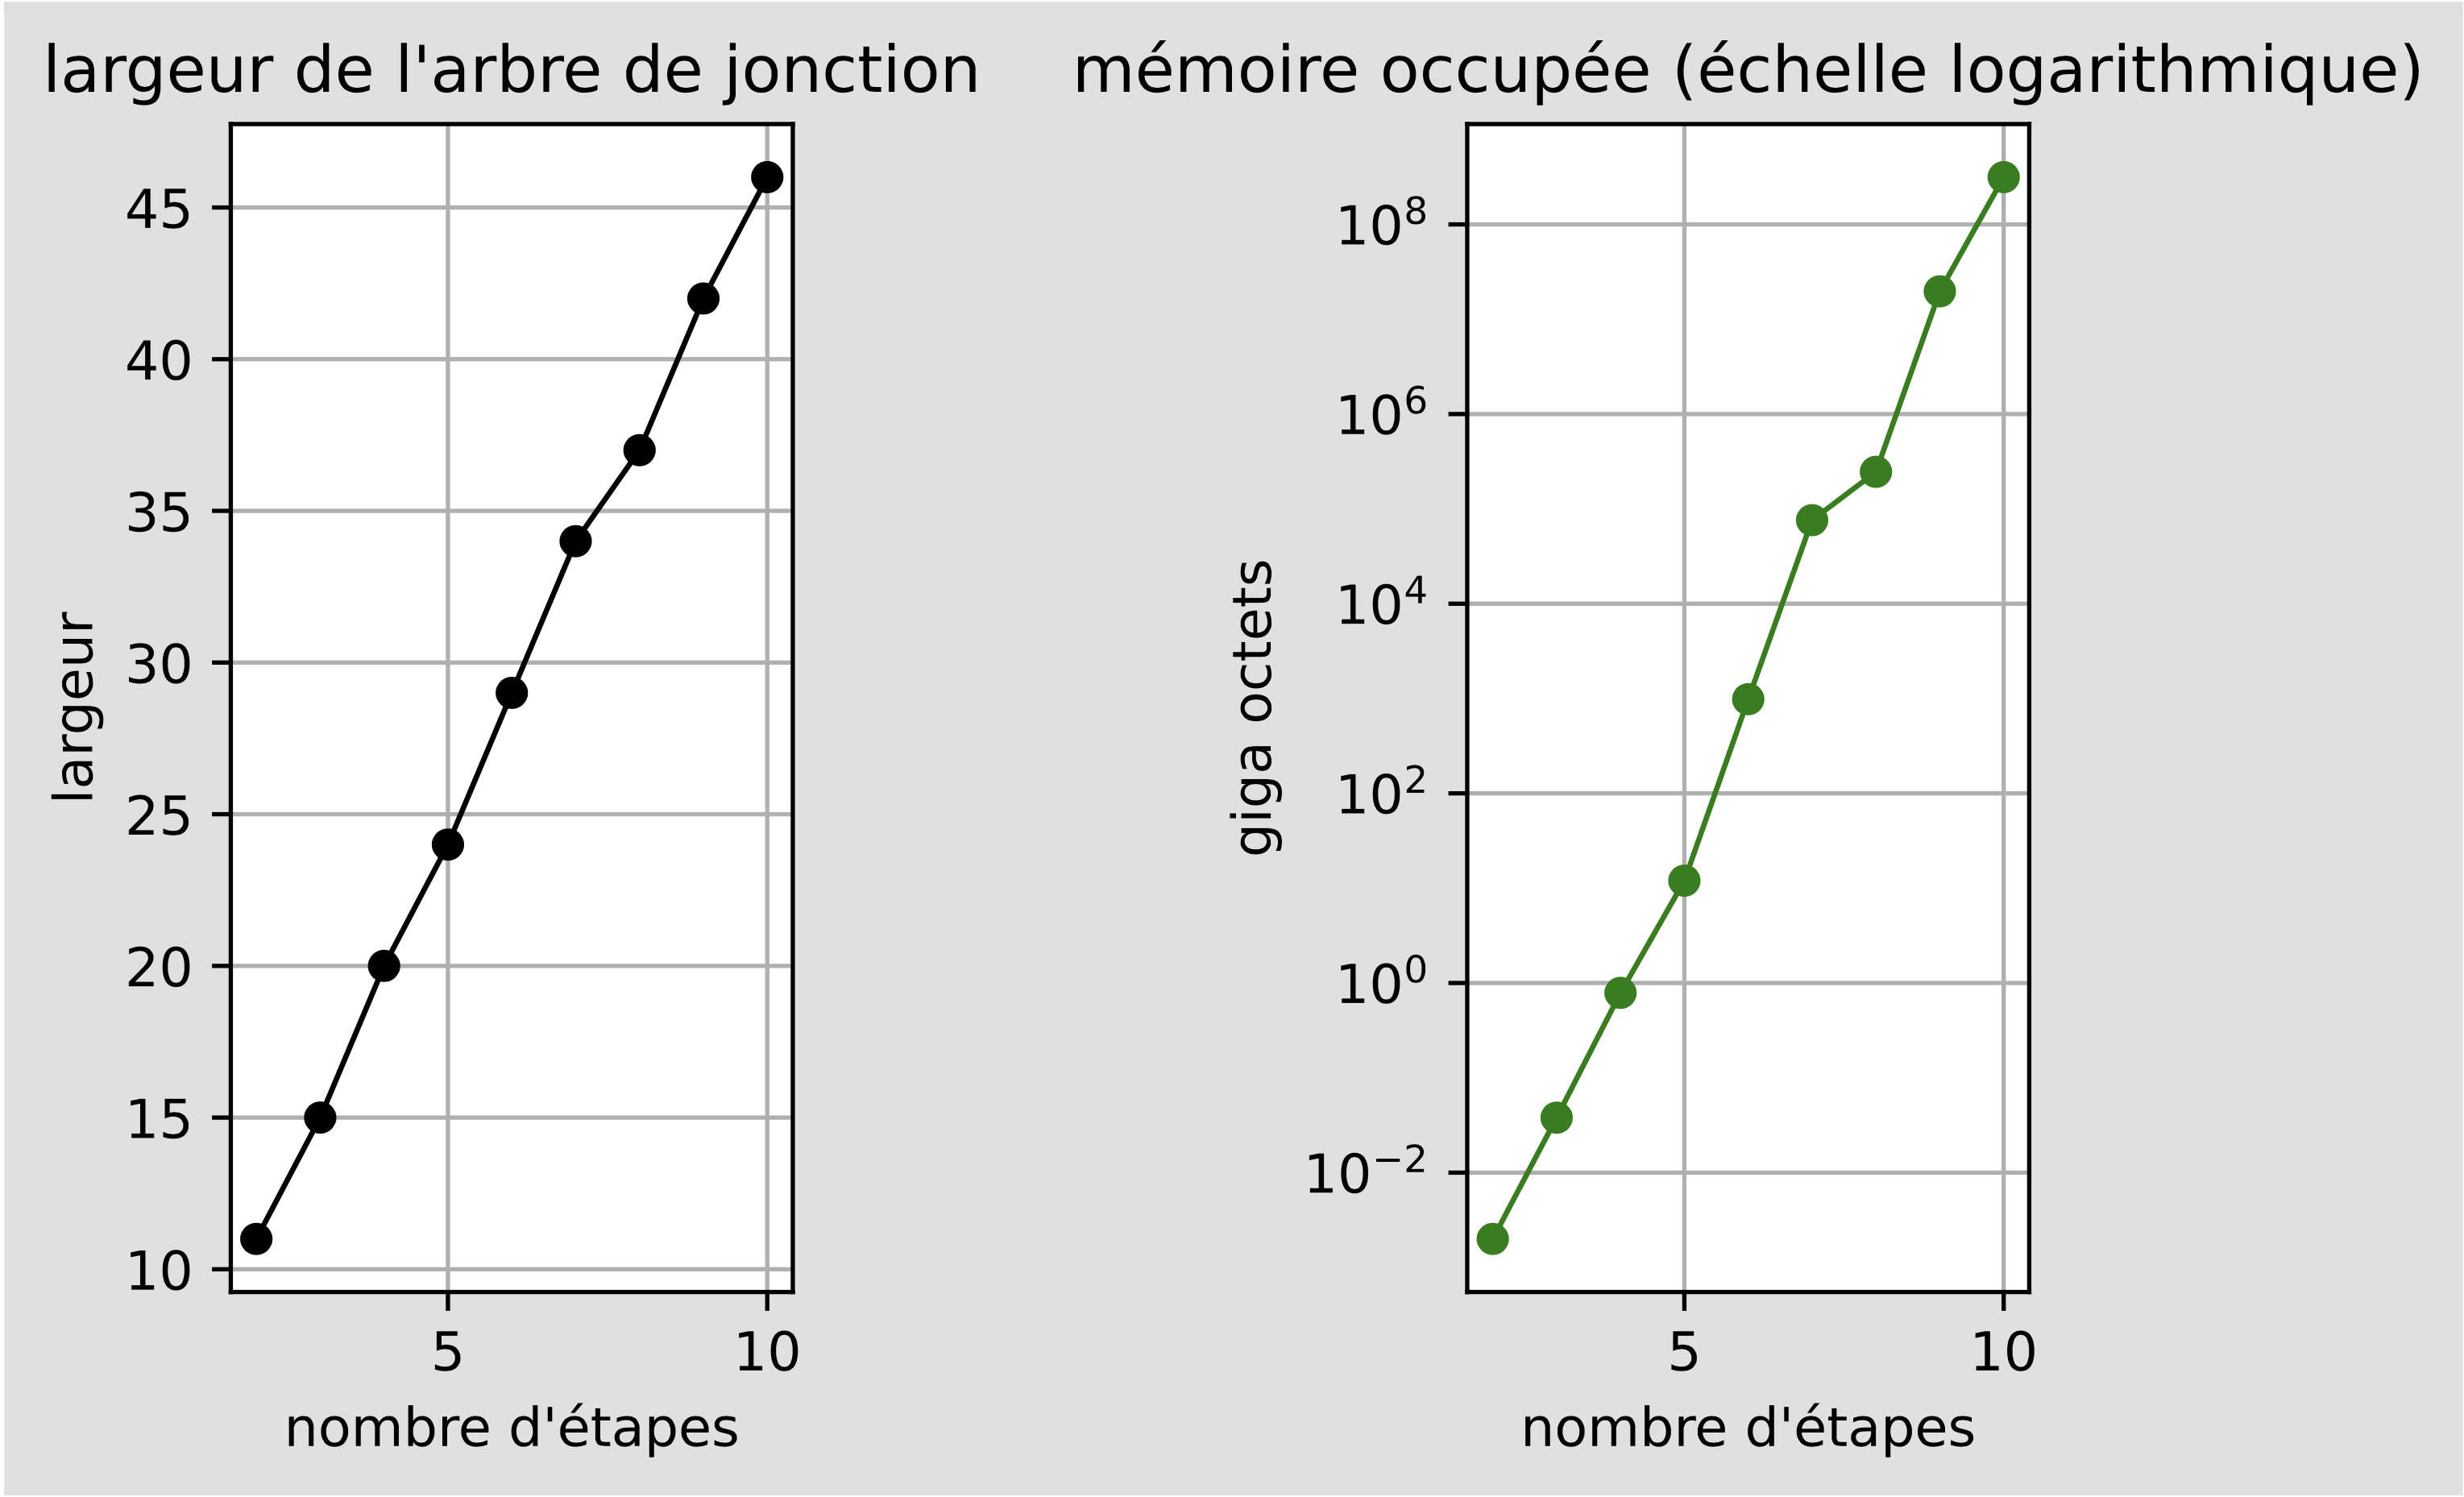
\includegraphics[scale=0.2]{docs/ressources_rapport/graphes.png}
\caption{Graphes sur la complexité en temps et espace des méthodes actuelles}
\end{figure}

On parvient à résoudre cet ID avec les méthodes exactes actuelles (une machine avec 128Go de mémoire vive) sur des instances du problèmes comprenant jusqu'à 5 étapes. Au delà de 5 étapes, la mémoire nécessaire et le temps pour trouver la solution explose. \bigbreak
Il n'est pas envisageable de concevoir une machine capable de stocker autant de données pour résoudre de façon exacte cet ID. Il y a donc un réel besoin d'avoir une implémentation permettant de résoudre plus rapidement les IDs et en nécessitant moins d'espace.
\bigbreak
\bigbreak
\pagebreak

\subsection{But du projet}
Ce projet avait un cadre prospectif et était orienté recherche. Ni nous ni notre encadrant ne savions quels en serait les aboutissants. Pour mener à bien ce projet, nous avons donc d'abord eu besoin de nous familiariser avec le sujet et de trouver les documents adéquats pour répondre à nos questions. Après cela, nous avions donc pour but d'étudier et d'implémenter un algorithme de Branch and Bound pour résoudre des LIMIDs afin de proposer une solution à l'explosion en espace des algorithmes actuels. Nous nous appuierons fortement sur les travaux de Yuan et Hensen [4], et d'Acid et Campos [6] qui posent les bases et explicitent les étapes de construction de l'algorithme. Celui-ci devra être documenté et testé.
Enfin, il est envisagé d'intégrer l'algorithme dans la librairie Python PyAgrum.

Ce sujet d'implémentation étant orienté recherche, nous n'avons pas de réel cahier des charges et avons décidé de l'inclure directement à ce rapport. Ce dernier correspond à la partie 4.1.    


\section{Algorithme de Branch and Bound pour la résolution de LIMIDS}
\subsection{Description informelle}
Les LIMIDs sont résolus en trouvant une stratégie qui maximise l'utilité prévue.
L'algorithme étudié dans ce projet résout les LIMIDs en les convertissant en un graphe ET/OU puis en effectuant un parcours en profondeur sur ces derniers.

Les nœuds ET sont alors des variables aléatoires correspondant aux nœuds chances qui sont informatifs à un nœud de décision et les nœuds OU sont des nœuds de décision (représentant des alternatives de décision), enfin les feuilles sont les nœuds d'utilités.

Durant le parcours en profondeur, un chemin racine-feuille représente une instance des nœuds d'information et de décision. Ces nœuds sont générés à la volée, ce qui permet de limiter l'utilisation de la mémoire. Les bornes supérieures et les évaluations des solutions candidates sont aussi calculées à la volée, permettant d'élaguer les chemins non prometteurs. Les calculs des bornes supérieures sont faites sur un ID relaxé, dont la construction est détaillée plus tard dans le rapport.

Il faut souligner que cet algorithme n'applique pas classiquement le Branch and Bound comme dans le problème du sac à dos par exemple (où les nœuds sont des sacs avec plus ou moins d'objets)dont une branche peut être élaguée si une solution courante est meilleure que la borne supérieure de cette branche. 

En effet, l'élagage se produit uniquement sur les branches sortant de nœuds de décision (ceux qui ne sont pas des feuilles) et non tous les nœuds. L'arbre se compose  aussi de nœuds chances mais on ne peut pas élaguer leurs branches car ces nœuds construisent toutes les instances possibles du LIMID. On élague donc seulement sur les branches sortant des nœuds de décision car leurs évaluations sont commensurables puisqu'elles ont le même contexte. En contrepartie, un nœud de décision ne peut pas faire élaguer une branche d'un autre nœud de décision car elles ne possèdent pas le même contexte : si une branche d'un nœud de décision est élaguée car un autre nœud de décision est mieux évaluée, c'est une alternative du LIMID qu'on n'exploreras pas et donc on ne va pas résoudre entièrement le LIMID.


\subsection{Implémentation des arbres ET/OU}
Les implémentations actuelles des arbres ET/OU ne sont pas satisfaisantes au regard des besoins de l'algorithme, nous avons donc implémenté notre version de l'arbre. Cette implémentation contient trois classes : une classe modélisant un graphe ET/OU, une classe modélisant les nœuds ET (nœuds de chance) et enfin une classe modélisant les nœuds OU (nœuds de décision).

Dans l'arbre ET/OU, un nœud OU (décision) est créé pour chaque alternative d'instancia\-tion des nœuds chances parents de ce nœud, et cela pour tous les nœuds de décision différents dans l'ID. C'est-à-dire que chaque nœud de décision dans l'ID a plusieurs contextes de nœuds chances possibles et tous sont représentés dans le graphe ET/OU par un nœud OU correspondant, à la suite du chemin des nœuds ET correspondants au contexte. Notre arbre se structure donc en couche, chaque couche étant constituée du même nœud de décision plusieurs fois (une fois par contexte possible) précédé de ses nœuds parents chance instanciés. 

Ensuite, chaque nœud de décision va construire à la volée des branches au nombre égal, au maximum, au nombre de possibilités de décision de ce nœud (au maximum car il peut y avoir élagage). Ces fils vont être structurés de la même manière que précédemment en créant tous les contextes possibles pour le prochain nœud de décision. Soulignons encore qu'on ne peut ainsi pas élaguer entre nœuds de couches différentes mais seulement entre fils d'un même nœud de décision.

La structure détaillée de l'implémentation est accessible en annexe.

\subsection{Implémentation de l'algorithme}

\subsubsection{ID relaxé et calcul des bornes}
Pour permettre l'élagage, nous devons calculer les bornes supérieures et inférieures pour toute les valeurs d'instantiation possibles des nœuds de ET (décision).La borne inférieure est la meilleure valeur courante calculée pour un nœud OU.
Pour sa borne supérieure, il faut résoudre un ID relaxé. 
Ce dernier est créé en ajoutant des informations à l'ID de départ et en simplifiant l'ID en supprimant les arcs non requis. 
\bigbreak
Les informations ajoutées sont sous la forme d'arcs entre des nœuds d'information et des nœuds de décision. Pour savoir quels arcs à ajouter à un nœud de décision, il faut calculer son \textit{sufficient information set} (SIS).
\bigbreak
L'ID relaxé est alors crée en deux étapes :
tout d'abord, le SIS de chaque nœud de décision est calculé dans l'ordre temporel inverse des décisions (donné par le décideur) $D_n$, ..., $D_1$ faisant de chaque nœud chance dans leur SIS correspondant un de leur nœud parent.
Enfin, les arcs d'information non requis sont supprimés de l'ID.

\subsubsubsection{Sufficient Information Set (SIS)}
Le calcul du SIS a été un point majeur de l'implémentation de l'algorithme et nous a pris une grande partie du temps alloué au développement.
\bigbreak
Nous nous sommes basé sur l'article d'Acid et Campos [6] qui propose une méthode basé sur l'algorithme de Ford et Fulkerson afin de trouver l'ensemble séparant entre deux nœuds dans un graphe non dirigé et l'article de Yuan et al. [4] qui nous proposé les ensembles de nœuds sur lesquels appliquer l'algorithme.
\bigbreak
Nous avons implémenté 3 versions de l'algorithme :
\begin{itemize}
    \item La première se basait sur la construction complète d'un graphe auxiliaire à partir de l'ID, sur lequel on pouvait appliquer Ford et Fulkerson.
    \item La deuxième, plus performante, utilisait quant à elle un algorithme sur un graphe moralisé ancestral où on applique Ford et Fulkerson de manière implicite.
    \item La troisième, dont la majorité du code a été fourni par M. Wuillemin, était similaire au deuxième jet mais en présentant des optimisations et un code plus propre.
\end{itemize}
Nous soulignons le fait que la compréhension des articles était délicat, d'une part à cause de notre inexpérience sur ce sujet et d'autre part à cause de l'écriture confuse et expéditive de la part d'Acid et Campos [6]. L'implémentation de cet algorithme est complète mais il reste des points confus qui restent à discuter tel que le choix final des nœuds dans le SIS, la méthode de parcours du graphe moralisé ancestral dans certaines parties de l'algorithme ou encore la validité de la théorie derrière l'adaptation de l'algorithme Ford and Fulkerson. Il est d'autant plus important pour le projet de bien comprendre cette partie au vu de l'importance d'une relaxation informative du diagramme d'influence.

\subsubsection{Branch and bound}
Après avoir construit l'ID relaxé, nous pouvons commencer à appliquer l'algorithme. 

L'idée de départ était d'appliquer un Branch and Bound sur un \textit{graphe} ET/OU construit à partir d'un LIMID donné, d'évaluer les solutions candidates et de calculer les bornes supérieures avec un algorithme itératif utilisant les arbres de jointures fort construit eux aussi à partir de l'ID. 
\bigbreak
Par manque de temps, nous nous sommes résolus à :
\begin{itemize}
    \item Utiliser un arbre ET/OU au lieu d'un graphe ET/OU. En effet, l'idée originale était de construire un graphe ET/OU au lieu d'un arbre ET/OU pour la résolution de LIMID car ils offraient des optimisations en temps et en espace en exploitant le fait que, dans un LIMID, comme l'assomption du non oubliant est assoupli, beaucoup de décisions seront prises dans le même contexte. Ce qui augmenterait à la fois le temps de calcul en faisant des inférences plusieurs fois, mais aussi l'espace requis car on doit stocker plus de nœuds. Le graphe ET/OU devait en plus des nœuds ET et OU, avoir des nœuds spéciaux qui facilite l'implémentation de l'algorithme.
    \item Calculer les bornes supérieures et les évaluations avec de l'inférence exacte complète à chaque fois, ce qui augmente grandement notre complexité en temps (qui va même devenir le goulot d'étranglement de l'algorithme).
\end{itemize}

Nous devons donc commencer par construire l'arbre ET/OU, et ce à la volée. Pour cela, nous commençons par choisir dans l'ordre de décision donné avec le LIMID, le premier nœud de décision $d_0$.

Nous générons alors les alternatives possibles d'instanciations des parents de $d_0$ que nous appellerons \textit{couche} de $d_0$. Cette couche est composée de nœuds ET (chance), nous ajoutons alors des nœuds OU (décision) correspondant à $d_0$ sur les feuilles de cette couche. Pour exemple, si $d_0$ est le nœud (6) de décision dans l'ID de la figure 2, ses parents sont $ns_0, es_0, ss_0, ws_0$. Ceux-là ont pour domaine $[True, False]$  dont il y a $2^4=16$ alternatives possibles pour $d_0$.
%mettre l'arbre généré par l'exemple du robot
Lorsque cela est fait, s'il y a plus d'un seul nœud de décision dans le LIMID, nous calculons la borne supérieure des nœuds OU générés (pour toutes les valeurs de son domaine) et nous générons la couche pour les nœuds de décision suivants dans l'ordre de décision donné pour une branche d'un des nœuds OU qu'on vient de créer (on garde en mémoire, pour les nœuds OU, quelles branches ont été développées, évaluées, ou élaguées). Lorsque nous arrivons au dernier nœud de décision, il faut faire une inférence pour tous les nœuds de décision de cette couche feuille, pour tous les éléments de domaines de ces nœuds afin qu'on puisse remonter par un processus similaire à l'induction arrière dans la résolution d'un arbre de décision (la valeur d'un nœud chance est la moyenne pondérée par les probabilités postérieures des valeurs de ses fils et la valeur d'un nœud de décision est le maximum des valeurs de ses enfants). Lorsque cette induction arrière qui remonte la couche atteint son nœud de décision père, nous pouvons regarder si on peut élaguer en comparant les bornes supérieures des autres branches du nœud de décision avec l'évaluation de la couche (on met aussi à jour la meilleure solution courante pour ce nœud de décision s'il le faut). Lorsque un nœud de décision a toutes ses branches évaluées ou élaguées, il est \textit{processed}. Lorsque tous les nœuds de décision dans une couche sont \textit{processed}, nous pouvons faire l'induction arrière pour cette couche. Nous répétons ces étapes jusqu'à atteindre la racine de l'arbre ET/OU. 

Si, par contre, il n'y a qu'un seul nœud de décision, la première couche est alors une couche feuille dans l'arbre ET/OU et nous procédons comme dans le premier cas.

À la fin d'une exécution, nous avons donc un arbre ET/OU dont les nœuds de décision ont une décision optimale et une valeur d'utilité pour cette décision, les nœuds chances ont des probabilités postérieures associées ainsi qu'une valeur. Nous avons donc calculé pour toutes les alternatives une décision optimale.
%L'arbre de jointure est construit à partir de l'ID relaxé et est utilisé pour calculer les probabilités et les bornes supérieures pour le graphe ET/OU.
% \subsection{Extension aux LIMIDs}
%L'algorithme pour résoudre un ID utilise un arbre ET/OU, à la différence de celui résolvant un LIMID qui, lui, utilise un graphe ET/OU.
%Afin d'étendre l'approche Branch and Bound aux LIMIDs, on utilise un algorithme d'arborescence de jointure.
\subsection{Test}
Nous avons écrit plusieurs test unitaires, notamment pour tester l'algorithme de calcul du SIS. Celui-ci calcule en réalité l'ensemble séparant minimal dans un réseau bayésien. Nous avons donc testé sur des réseaux bayésiens générés aléatoirement si l'ensemble séparant minimal de deux nœuds tirés au hasard font bien de ces deux nœuds des nœuds indépendants. Nous avons aussi testé le branch and bound sur des IDs aléatoires afin de vérifier qu'il prenne en charge tous types de diagrammes.

\subsection{Documentation}
Une documentation des classes et des méthodes est disponible en annexe sous format PDF, elle a été rédigée en anglais dans le style numpy. Une version en ligne est aussi disponible sur \url{https://davidpinaud.github.io/PANDROIDE_InfDiag_BandB/}
\section{Évaluation de l'algorithme Branch and Bound}
\subsection{Performances en temps}
Sur l'exemple de la figure 2, l'ID relaxé construit avec les SIS était mauvais et donnais des valeurs (les bornes supérieures) de MEU très élevées comparés aux évaluations des solutions candidates. Il n'y avait donc pas d'élagage possible et l'exécution était très longue : 25 minutes comparé à moins d'une seconde avec la méthode classique.

La performance en temps dépend largement de la qualité de la relaxation et donc de la borne supérieure qui influe directement sur le nombre d'inférence à faire par les élagages qu'elle permet. Elle est aussi très impacté par le fait que nous avions choisis de faire des inférences exactes à chaque calcul de bornes ou d'évaluation au lieu d'implémenter la méthode itérative.

Les performances en temps du branch and bound comparé à l'algorithme Shafer Shenoy sont mauvaises aussi. Ce dernier est exponentiellement plus rapide proportionnellement au nombre de noeuds et d'arcs dans le LIMID. Ceci est peut être dût à la mauvaise optimisation de notre code, couplé aux concessions sur l'algorithme initial décidé, mais aussi dû au fait que le branch and bound a été écrit en Python et l'implémentation de l'algorithme de Shafer Shenoy en C++.
\subsection{Performances en espace}
La performance en espace de notre algorithme dépend largement de la structure du LIMID. 
En effet, l'arbre est d'autant plus profond qu'il y a de nœuds de décision et d'autant plus large que le nombre de parents des nœuds de décision et leur domaine. Nous rappelons aussi que la performance en espace est impacté par notre choix d'utiliser des arbres ET/OU et non des graphes ET/OU. Elle dépend aussi des potentiels des nœuds et de la qualité du relaxé : plus le relaxé est bon, plus on élaguera. 

À titre de comparaison avec l'exemple de la figure 2, voici le nombre de nœuds crée et la quantité de mémoire occupée dans le graphe ET/OU en fonction du nombre de stages.

\begin{figure}[ht]
\centering
\begin{subfigure}{.5\textwidth}
  \centering
  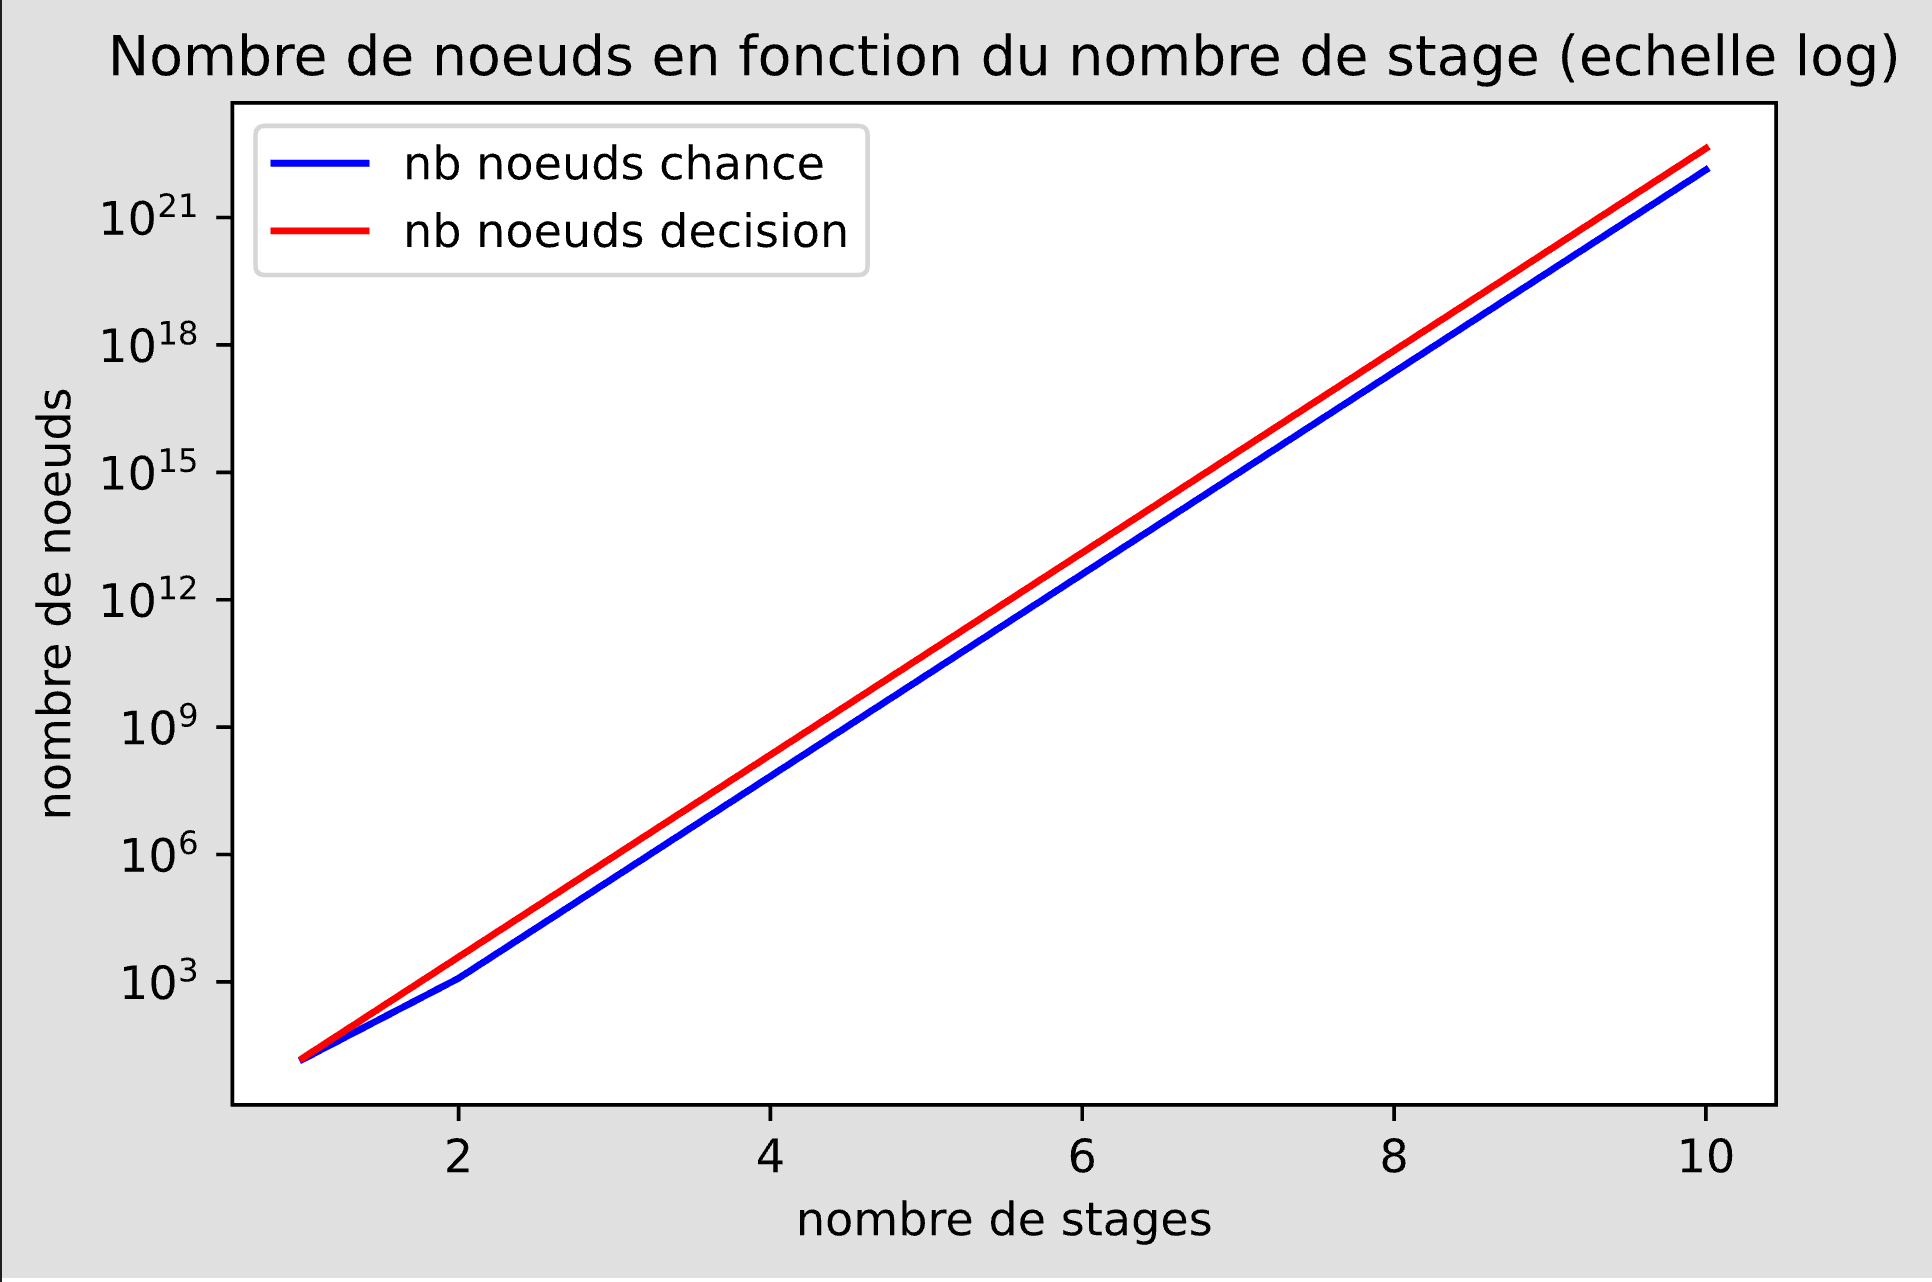
\includegraphics[width=.65\linewidth]{docs/ressources_rapport/perf_espace.png}
  \caption{Nombre de nœuds/Stage}
  \label{fig:sub8}
\end{subfigure}%
\begin{subfigure}{.5\textwidth}
  \centering
  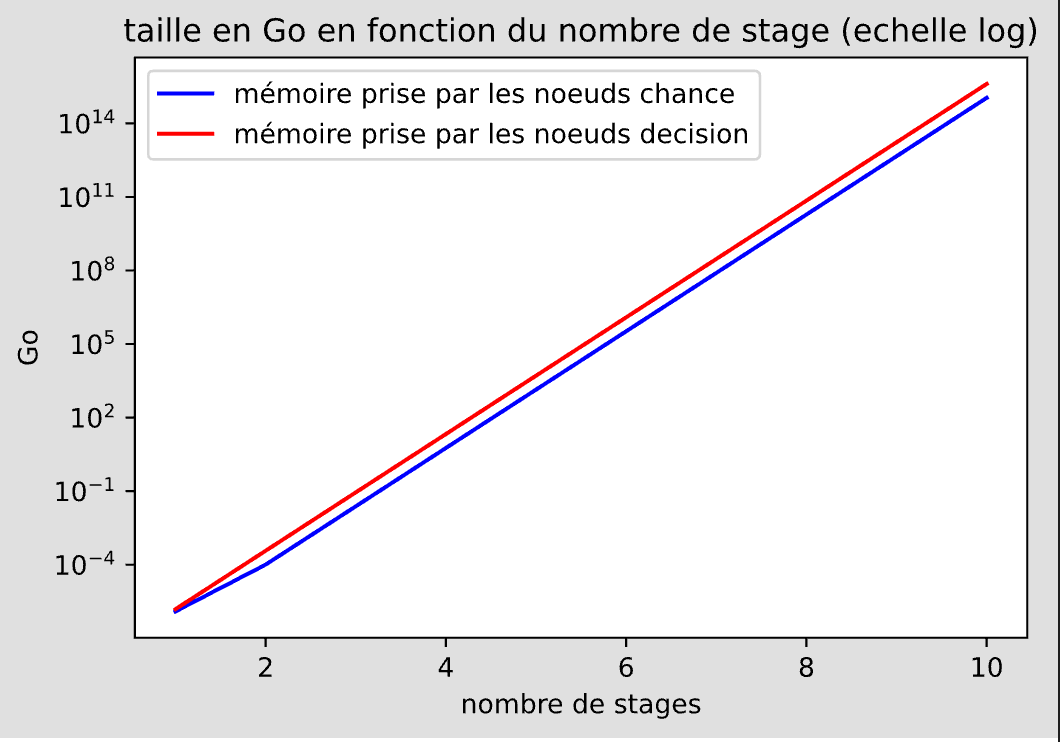
\includegraphics[width=.65\linewidth]{docs/ressources_rapport/perf_Go.png}
  \caption{Mémoire/Stage}
  \label{fig:sub9}
\end{subfigure}
\caption{Performance en espace}
\label{fig:test4}
\end{figure}

Remarquons que c'est la même complexité exponentielle que les algorithmes de résolutions actuels qui ressort. C'est parce que le LIMID relaxé n'était pas informatif et aucun élagage n'est fait ! Cet exemple souligne encore l'importance du relaxé, en effet, l'élagage peut théoriquement diminuer de façon drastique le nombre de branches exploré.
Sur des exemples ou des élagages ont pu être fait, nous observons une réductions souvent drastique (souvent plus de 40\%) de la quantité de mémoire occupée et du nombre de noeuds crée dans l'arbre ET/OU.
En comparaison directe avec l'implémentation de Shafer Shenoy en C++, le branch and bound occupe beaucoup plus d'espace sur le disque. Cette différence de performance est sûrement dû au choix du langage d'implémentation et de l'optimisation de l'algorithme.

\subsubsection{Exemples}
Voici des exemples illustrant les performances en temps et en espace et l'importance de l'élagage :
\subsubsubsection{Exemple 1}
\begin{figure}[ht]
\centering
\begin{subfigure}{.5\textwidth}
  \centering
  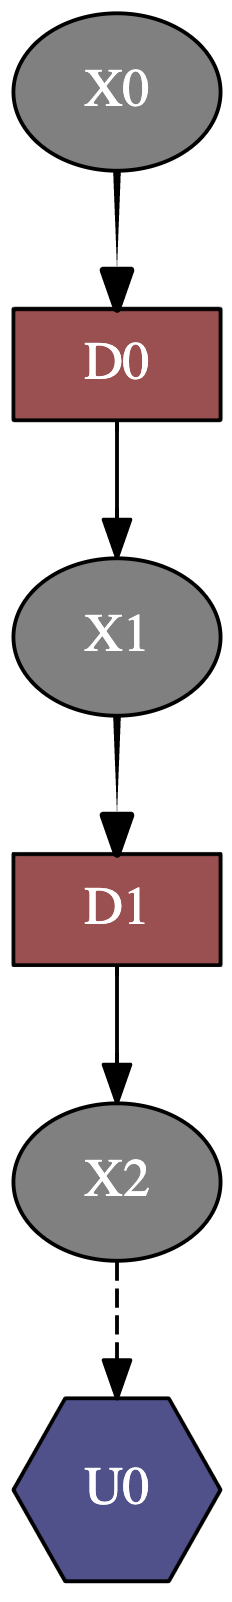
\includegraphics[width=.08\linewidth]{docs/ressources_rapport/ID_exemple.png}
  \caption{Diagramme d'influence}
  \label{fig:diag_inf}
\end{subfigure}%
\begin{subfigure}{.5\textwidth}
  \centering
  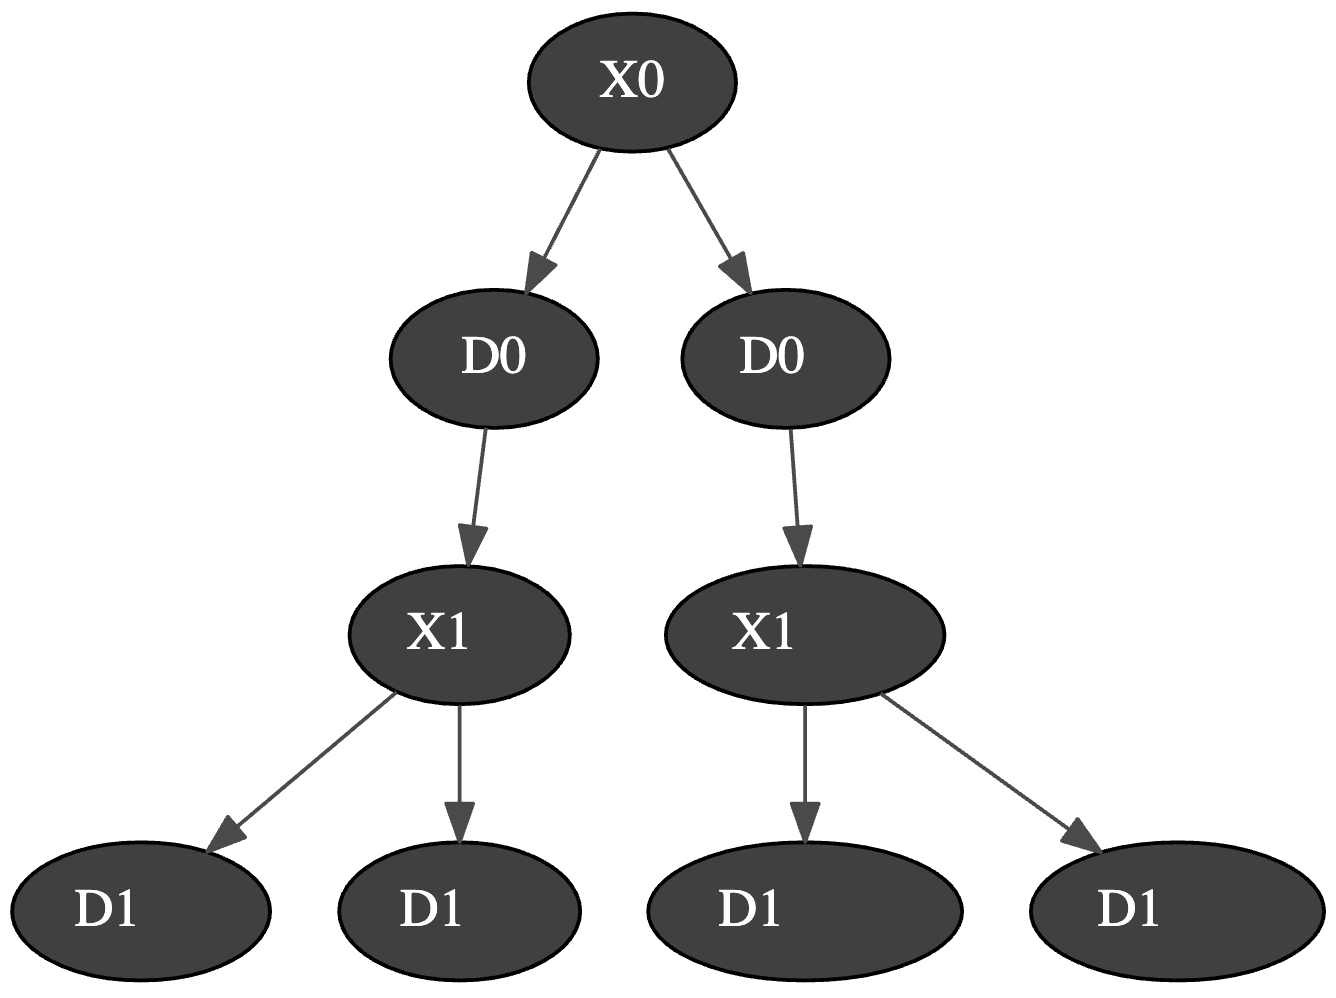
\includegraphics[width=0.75\linewidth]{docs/ressources_rapport/arbreETOU.png}
  \caption{L'arbre ET/OU construit pendant le branch and bound}
  \label{fig:arb}
\end{subfigure}
\caption{ID et Arbre ET/OU}
\label{fig:id_arbre}
\end{figure}

En effet, voici l'arbre ET/OU complet si aucun élagage n'est fait :
\begin{figure}[ht]
\centering
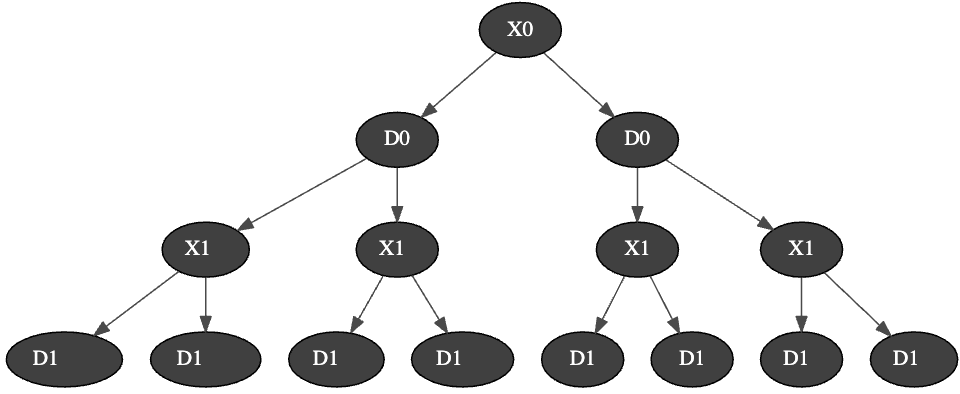
\includegraphics[width=1.\linewidth]{docs/ressources_rapport/arbreETOUComplet.png}
 \caption{Arbre ET/OU complet}
\end{figure}

Une branche des deux nœuds $D_0$ est élaguée, ce qui nous fait économiser la construction de 6 nœuds, représentant une économie d'espace de $40\%$. Cela nous libère aussi de $4\times 2=8$ calculs d'inférence exacte (fait sur les nœuds $D_1$), ce qui représente $50\%$ des calculs d'inférence et de deux remontées de sous-arbres (qui économise aussi du calcul car on n'a plus à calculer les valeurs des nœuds chances $X_1$ avec les probabilités à posteriori).

En comparaison avec l'inférence Shafer Shenoy, notre algorithme a fait l'inférence en 0.00956 secondes comparé à 0.00054 pour la méthode état de l'art soit $17,7$ fois plus rapide. 

Shafer Shenoy a construit un arbre de jonction de largeur 2 et a utilisé environ 32 octets de mémoire tandis que le branch and bound a utilisé un arbre ET/OU de profondeur 4 et environ 432 octets soit 32 fois plus d'espace occupé. Shafer Shenoy étant écrit en $C++$ et le branch and bound en Python, il est aisé de comprendre l'écart de performance entre les deux algorithmes.
\subsubsubsection{Exemple 2}
\begin{figure}[ht]
\centering
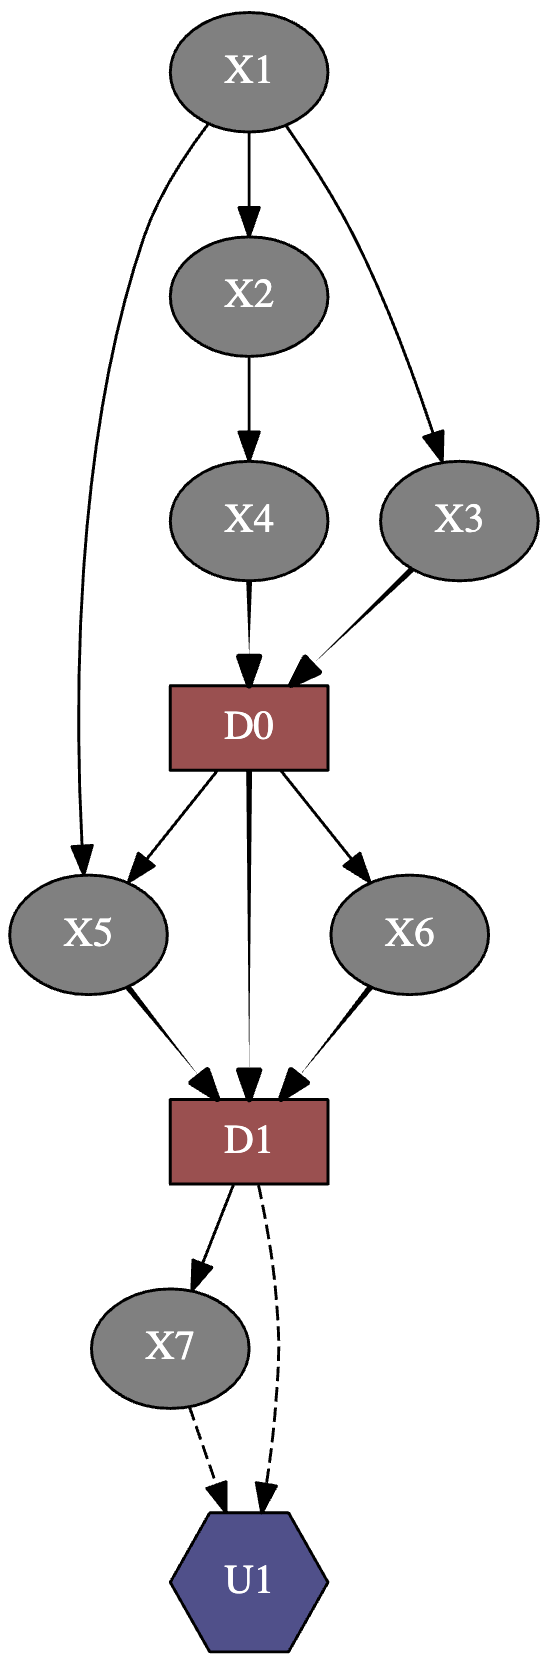
\includegraphics[width=0.2\linewidth]{docs/ressources_rapport/exempleID2.png}
 \caption{Diagramme d'influence}
\end{figure}

\begin{figure}[ht]
\centering
\begin{subfigure}{.5\textwidth}
  \centering
  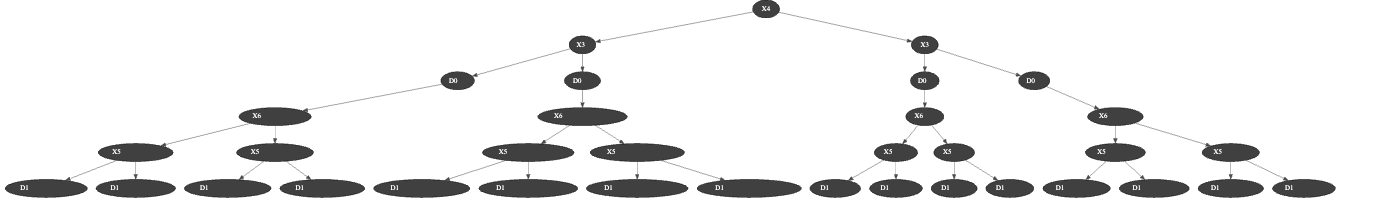
\includegraphics[height=40mm,width=1\linewidth]{docs/ressources_rapport/EXEMPLE2ANDOR.png}
  \caption{L'arbre ET/OU construit pendant le branch and bound}
  \label{fig:arbre}
\end{subfigure}%
\begin{subfigure}{.5\textwidth}
  \centering
  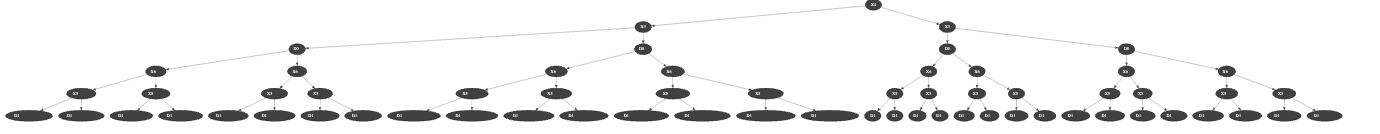
\includegraphics[height=40mm,width=1\linewidth]{docs/ressources_rapport/EXEMPLE2FULLANDOR.png}
  \caption{Arbre ET/OU complet}
  \label{fig:arbre_complet}
\end{subfigure}
\caption{Arbre ET/OU complet et élagué}
\label{fig:arbre_elague}
\end{figure}

Le branch and bound a élagué 4 branches, ce qui a permis de ne développer que 35 nœuds au lieu de 63 pour un temps d'exécution de 0.07885 secondes et un arbre de profondeur 6 occupant 1680 octets comparé à un arbre de jonction de largeur 3 occupant environ 64 octets et un temps d'exécution de 0.00126 secondes pour Shafer Shenoy. Le branch and bound est donc 204 fois plus lent et occupe 26 fois plus d'espace que la méthode actuelle.
\subsubsubsection{Exemple 3}
\begin{figure}[ht]
\centering
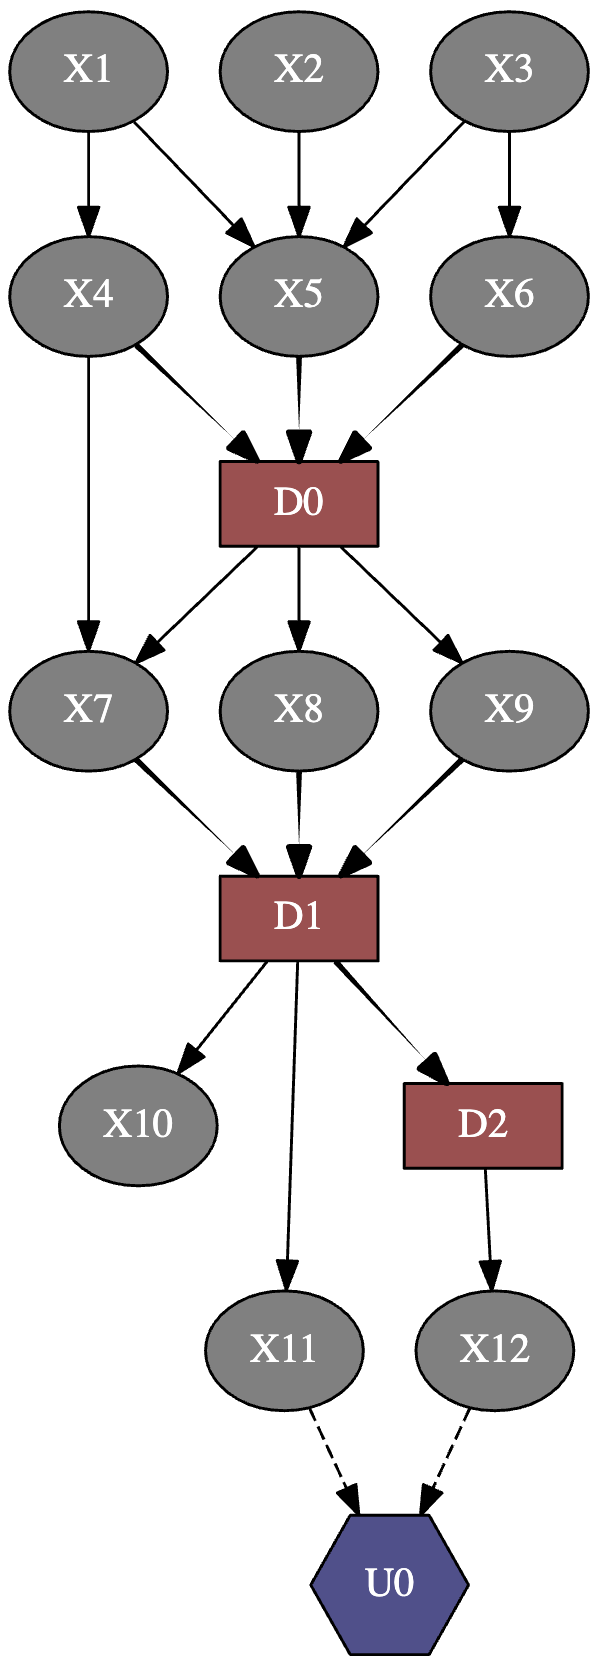
\includegraphics[width=0.2\linewidth]{docs/ressources_rapport/id3.png}
 \caption{Diagramme d'influence}
\end{figure}

Le branch and bound a élagué 8 branches, ce qui a permis de ne développer que 135 nœuds au lieu de 255 pour un temps d'exécution de 0.56199 secondes et un arbre de profondeur 7 occupant 6480 octets comparé à un arbre de jonction de largeur 4 occupant environ 128 octets et un temps d'exécution de 0.00275 secondes pour Shafer Shenoy. Le branch and bound est donc 62 plus lent et occupe 50 fois plus d'espace que la méthode actuelle.
\section{Intégration possible de l'algorithme dans PyAgrum}
% *vérifier la compatibilité de l'inférence avec les inférences existantes
% *vérifier la compatibilité avec notebooks
\subsection{Déliverables du projet}
Le projet a pour but de réaliser :
\begin{itemize}
\item Un état de l'art et stabilisation des algorithmes pour la résolution avec Branch and Bound, en particulier l'analyse du calcul des bornes et des probabilités postérieures.
\item Une implémentation efficace et compacte des arbres ET/OU.

\item Une intégration de l'algorithme correctement documentée (style python en anglais) dans l'API pyAgrum vérifiant l'implémentation des méthodes (liste non exhaustive) :
\begin{itemize}
    \item makeInference : Réalise l'inférence sur un LIMID.
    \item PosterieurUtility : Retourne la probabilité postérieure d'un nœud.
    \item LIMInfluenceDiagram : Retourne le LIMID associé à l'instance de la classe.
    \item optimalDecision : Retourne la décision optimale pour un certain nœud décision basée sur le critère MEU.
    \item MEU : Retourne l'utilité maximale espérée de l'inférence.
    \item junctionTree : Retourne l'arbre de jonction associé au LIMID
    \item andOrTree : Retourne le graphe de jonction développé
    \item une fonction pour visualiser l'arbre ET/OU
\end{itemize}
\item Une série de tests unitaires effectués sur les méthodes avec l'API TestUnit.
\item Une série de benchmark validant l'utilité de notre implémentation de la méthode branch and bound face aux méthodes existante.
\end{itemize}

\section{Conclusion}
En conclusion, après avoir testé les algorithmes actuels sur un exemple, nous avons implémenté un algorithme de résolution de LIMID basé sur le branch and bound qui prouve la promesse de performance en terme d'espace de ce type d'approche (et qui pourrait également l'être en terme de temps de calcul en utilisant un algorithme incrémental), malgré la faible performance en comparaison directe avec l'algorithme de Shafer Shenoy dû à l'optimisation insuffisante de notre code. 

Nous avons souligné le rôle majeur de la relaxation dans la performance de l'algorithme et montré que l'algorithme pour la création de celle-ci n'est pas encore très bien compris au vu des difficultés qu'on a rencontré pendant l'implémentation de l'algorithme de calcul de SIS.

Nous avons donc appris à avoir un œil critique sur les documents étudiés et nous avons pu approfondir des notions dans le domaine d'aide à la prise de décision ainsi que l'utilisation de la librairie PyAgrum.

Enfin, nous remercions M.Pierre-Henri Wuillement pour ses contributions et ses conseils sans lesquels nous aurions sans doute pas pu venir à terme de ce projet.
 



\newpage
\section{Bibliographie}
\begin{itemize}

\item [1] C.Yuan and E.Hansen, « Efficient Computation of Join\-tree Bounds for Systematic MAP Search. », IJCAI Int. Jt. Conf. Artif. Intell., p. 1989, janv. 2009. 

\item[2] D.Nilsson and S.Lauritzen, « Evaluating influence\-diagrams using LIMIDs », Proc. Sixt. Conf. Uncertain. Artif. Intell., janv. 2013.

\item[3] A.Khaled, E.Hansen, and C.Yuan, « Solving Limited-Memory Influence Diagrams Using Branch-and-Bound Search », Int. Symp. Artif. Intell. Math. ISAIM 2012, sept. 2013.

\item[4] C.Yuan, X.Wu, and E.Hansen, Solving Multistage\-Influence Diagrams using Branch-and-Bound Search. 2012, p. 700.

\item[5] R.Dechter and R.Mateescu, « AND/OR searchspaces for\-graphical models », Artif. Intell.,vol. 171, p. 73‐106, févr. 2007, doi: 10.1016/j.artint.2006.11.003.

\item[6] S.Acid and L.M.deCampos, « An Algorithm for Finding Minimum d-Separating Sets in Belief Networks », in Proceedings of the twelfth Conference of Uncertainty in Artificial Intelligence,
1996, p. 22.

\item[7] D.D.Maua, C.P.deCampos, and M.Zaffalon, « Solving Limited Memory Influence Diagrams », J. Artif. Intell. Res., vol. 44, p. 97‐140, mai 2012, doi: 10.1613/jair.3625.

\item[8] D.R.Morrison, S.H.Jacobson, J.J.Sauppe, and E.C.Sewell, « Branch-and-bound algorithms: A survey of recent advances in searching, branching, and pruning », Discrete Optim., vol. 19, p. 79‐102, févr. 2016, doi: 10.1016/j.disopt.2016.01.005.

\item[9] R.A.Howard, J.E.Matheson, and Strategic Decisions Group, Éd.,Readings on the principles and applications of decision analysis, Repr. Menlo Park, Calif: SDG, 1989.

\item[10] A.J. Myles, R. N. Feudale, Y. Liu, N. A. Woody, and S. D. Brown, « An introduction to decision tree modeling », J. Chemom., vol. 18, no 6, p. 275‐285, 2004, doi:
https://doi.org/10.1002/cem.873.

\item[11] D. Geiger, T. Verma, and J. Pearl, « d-Separation: From Theorems to Algorithms », in Machine Intelligence and Pattern Recognition, vol. 10, M. Henrion, R. D. Shachter, L. N. Kanal, et J. F. Lemmer, Éd. North-Holland, 1990, p. 139‐148.

\item[12]David Kahle, Terrance Savitsky, Stephen Schnelle, and Volkan Cevher, « Junction tree algorithm », Stat, Volume 631, 2008.
\end{itemize}

\newpage


\section{Annexes}
\subsection{Liens divers}
\underline{\textbf{Documentation : }}
\begin{itemize}
    \item WEB : \url{https://davidpinaud.github.io/PANDROIDE_InfDiag_BandB/}
    \item PDF : \url{https://github.com/davidPinaud/PANDROIDE_InfDiag_BandB/tree/master/docs/documentation}
\end{itemize}
\underline{\textbf{Carnet de Bord : }}
\begin{itemize}
    \item PDF : \url{https://github.com/davidPinaud/PANDROIDE_InfDiag_BandB/blob/master/docs/pdf/Carnet\%20de\%20bord.pdf}
\end{itemize}
\underline{\textbf{Dépendances : }}
\begin{itemize}
    \item Python >3.8.5 :\url{https://www.python.org/downloads/}
    \item PyAgrum >0.20.2 : \url{https://gitlab.com/agrumery/aGrUM/blob/0.20.2/wrappers/pyAgrum/doc/sphinx/index.rst}
    \item NumPy >v1.20.0 : \url{https://numpy.org/install/}
    \item pydotplus >2.0.2 : \url{https://pypi.org/project/pydotplus/}
    \item Matplotlib >3.4.1: \url{https://matplotlib.org/stable/users/installing.html}
\end{itemize}
\subsection{Structre des éléments de l'arbre ET/OU}
Les nœuds de décision ont pour attributs :
\begin{itemize}
\item Un identifiant au sein de l'arbre ET/OU
\item Un dictionnaire de contexte dont la clef est l'identifiant du nœud (dans le diagramme d'influence, ce qui est possible même s'il y a plusieurs nœuds correspondant au même nœud de décision, puisqu'on regarde le contexte dans l'ID et non pas dans l'arbre ET/OU) et dont la valeur est la valeur d'instanciation
\item Une valeur d'instanciation du nœud
\item Deux identifiants (celui du nœud correspondant dans l'ID pour retrouver à quel nœud dans l'ID celui ci corresponds, et un autre identifiant pour le graphe ET/OU)
\item Une liste de parents.
\item Un dictionnaire de bornes supérieures dont la clef est la valeur du domaine et dont la valeur est un tuple (moyenne, variance).
\item Un dictionnaire d'enfants dont la clef est la valeur du domaine et dont la valeur est l'enfant, un dictionnaire d'évaluations dont la clef est la valeur du domaine et dont la valeur est un tuple (moyenne, variance).
\item Un support (domaine du nœud).
\item Une décision optimale (une valeur du domaine du nœud de décision).
\item La valeur de cette décision (la moyenne du MEU).
\item Une liste de nœuds élagués.
\item L'inférence qui a été faite sur l'instanciation qui a mené à ce nœud.
\item La liste des enfants qui ont été évalués.
\end{itemize}
Les nœuds de chance ont pour attributs :
\begin{itemize}
\item Un identifiant.
\item Un support.
\item Un dictionnaire d'enfants dont la clef est la valeur du support et dont la valeur est l'enfant.
\item Une valeur d'instanciation, une liste de parents, et leurs valeurs.
\item Un dictionnaire de probabilités postérieures dont la clef est la valeur du support et dont la valeur est la probabilité.
\item Un dictionnaire de contexte dont la clef est l'identifiant du parent, et dont la valeur est le domaine.
\item Un identifiant au sein de l'arbre ET/OU.
\end{itemize}

L'arbre (classe andOrGraph) a pour attributs :
\begin{itemize}
\item Le diagramme d'influence que l'on utilise pour l'arbre ET/OU.
\item Un nœud chance racine.
\item Une liste de nœuds.
\item Une liste de nœuds chance.
\item Une liste de nœuds de décision.
\item Un identifiant au sein de l'arbre ET/OU.
\end{itemize}
\subsection{Documentation version PDF (voir page suivante)}
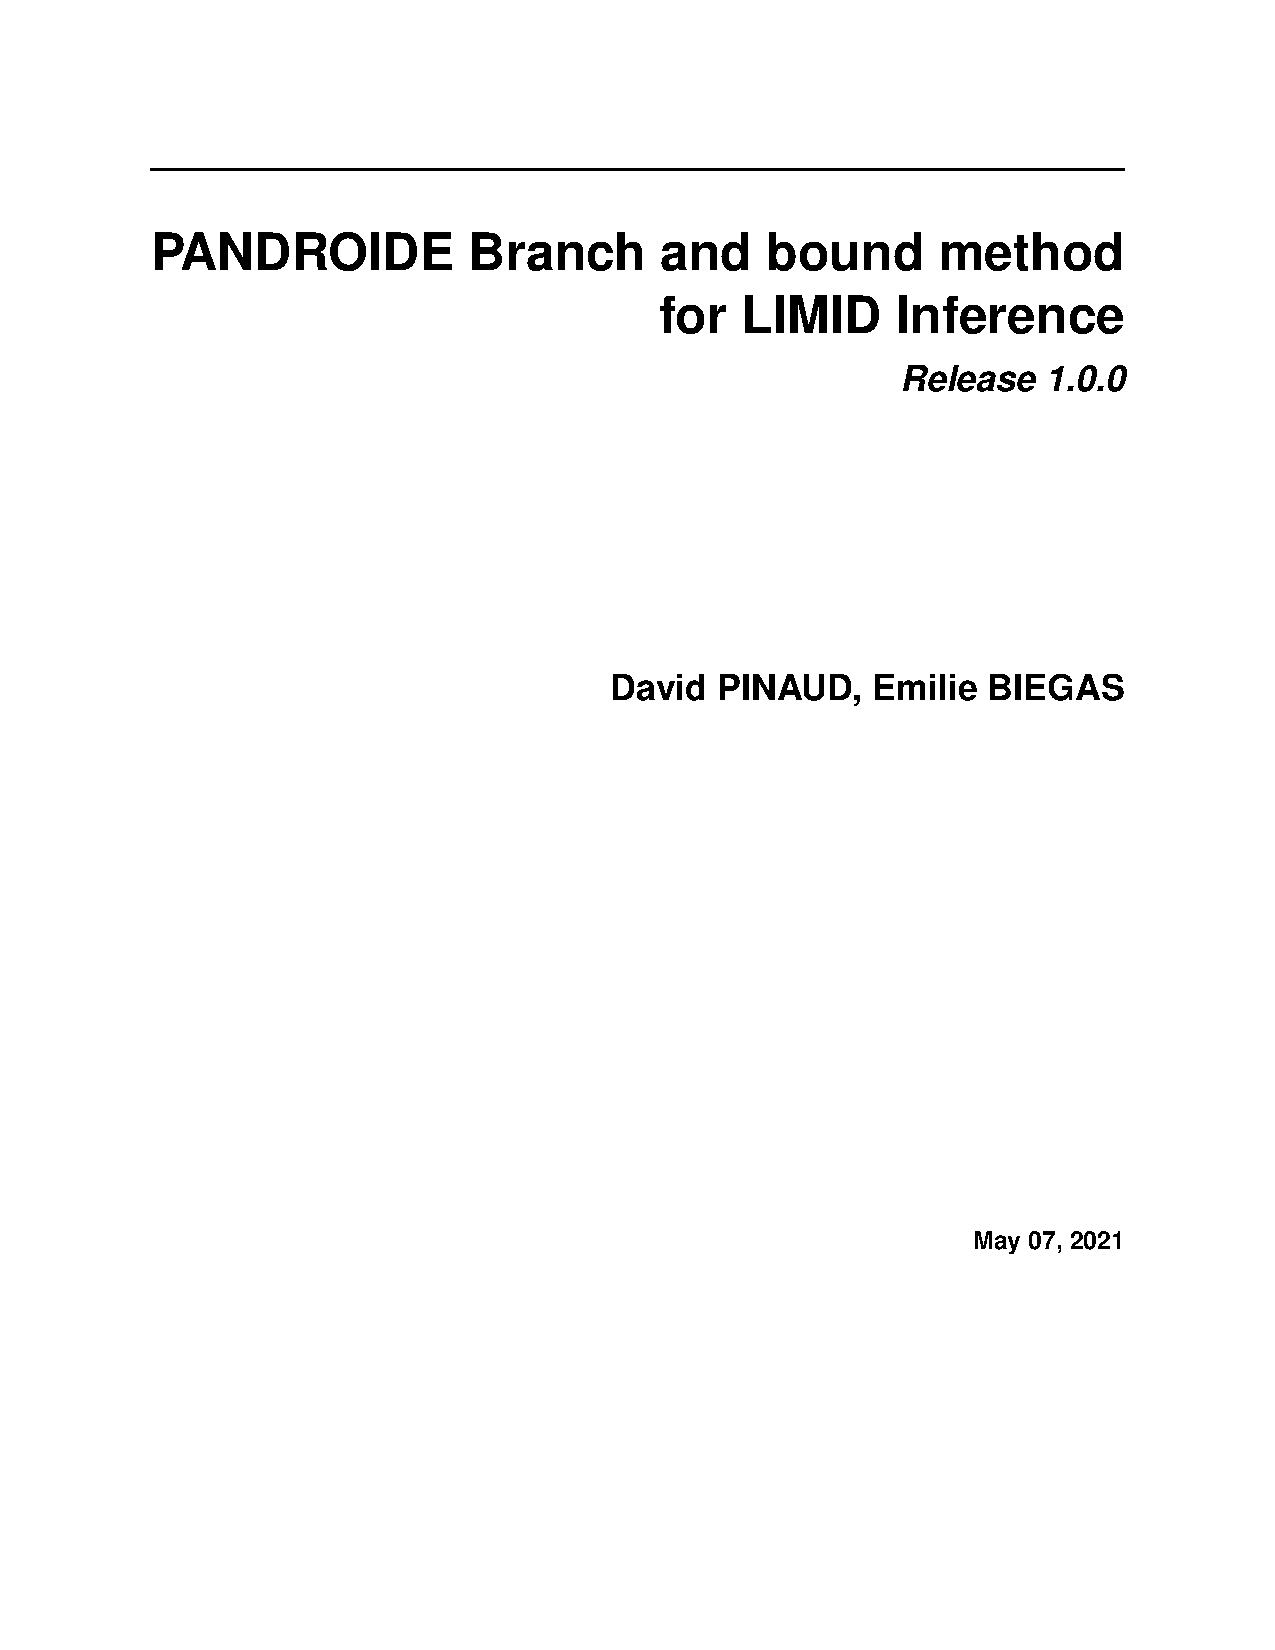
\includepdf[pages=-]{../documentation/doc_pdf/documentation.pdf}
\end{document}